\documentclass[10pt]{article}
\usepackage{amsmath} 
\usepackage{graphicx}
\usepackage{caption}
\usepackage{subcaption}
\usepackage{hyperref}
\usepackage{textcomp}
\usepackage{abstract}
\usepackage{mathtools}
\usepackage[normalem]{ulem}
\usepackage{fancyvrb}

\captionsetup{font=scriptsize}
\setlength{\columnsep}{15pt}

%% Adjustments
\renewcommand{\abstractnamefont}{\normalfont\normalsize\bfseries}
\renewcommand{\abstracttextfont}{\normalfont\it}
\setlength{\absleftindent}{0pt}
\setlength{\absrightindent}{0pt}

%% Note that anything in a LaTeX file which is preceded (on the same line)
%% by a % is a comment, and is totally ignored by LaTeX.

%% Next is the command to input the macro package which we shall use
%% for displaying Encapsulated Postscript figures

\input BoxedEPS


%%%%%%%%%%%%%%%%%%%%
%%
%% Depending on what operating system you are using, you need to
%% use one or other of the following two lines. Keep the one you
%% are NOT using ```commented out'', ie preceded by %.

%\SetTexturesEPSFSpecial  %% use this for the Mac & Textures
\SetRokickiEPSFSpecial  %% use for xdvi, dvips; i.e., for VMS, Unix, Athena

%% (These commands tell each computer platform how to invoke the %% TeX ``special'' command; see BoxedEPS.doc for details if you wish,
%% but I would not bother if I were you. KR.)
%%
%%%%%%%%%%%%%%%%%%%


\HideDisplacementBoxes

%% Hides the rectangular bounding box of the eps file;
%% comment this out if you want to see how large
%% the figure REALLY is -- i.e., there may be stray points . . .

%%%%%%%%%%%%%%%%%%%
%%
%% The next few lines are formatting commands. You must leave
%% these exactly as they are. (For your information, %% when your papers are turned into a book, these formatting
%% commands will be changed. The final published version will be in 10pt
%% type with somewhat different margins, designed to make it look good
%% as a book rather than as a document printed on 8.5 by 11 inch
%% paper. The page count will remain approximately the same.)



%%
%%%%%%%%%%%%%%%%%%%



%%
%%%%%%%%%%%%%%%


\begin{document}
\title{Assignment 1: 3D Photography using Planar Shadows}
\author{B. Tyler Parker\\
\small Brown University Computer Science Department\\
\small Providence, RI 02912\\
\small May 2013\\[-0.25in]} \date{} %% You could use \date{\small\today\today} to keep track
%% of preliminary versions
\maketitle


\section{Introduction}
For this assignment, we were tasked with creating a 3D scanner using shadow planes. I decided to re-implement the project in C++, using the openFrameworks framework and OpenCV library with OpenGL for 3D drawing.

\section{Camera Calibration}
Intrinsic parameters were obtained by using checkerboard detection in OpenCV, a benefit being that it was a fully automated and fast process. The sub-corners for the detected checkerboard corners are also computed. Two remap images (x and y distortions), generated from the distortion parameters, are used to then correct camera distortion in subsequent scanning frames.
\begin{figure}[h!]
  \centering
\begin{subfigure}[b]{\linewidth}
\centering
$fc = \begin{bmatrix}
   2063.50806 & 2068.35986\\[0.3em]
 \end{bmatrix}
 $
 \end{subfigure}
 \begin{subfigure}[b]{\linewidth}
 \centering
$cc = \begin{bmatrix}
   564.230042 & 424.529755 \\[0.3em]
 \end{bmatrix}
 $
 \end{subfigure}
  \begin{subfigure}[b]{\linewidth}
 \centering
$alpha\_c = \begin{bmatrix}
   0 \\[0.3em]
 \end{bmatrix}
 $
 \end{subfigure}
  \begin{subfigure}[b]{\linewidth}
 \centering
$kc = \begin{bmatrix}
   -0.165351689 \\[0.3em]
   0.263898373 \\[0.3em]
   0.00600361405 \\[0.3em]
   0.00365240709 \\[0.3em]
   11.0719986 \\[0.3em]
 \end{bmatrix}
 $
 \end{subfigure}
      \caption{Intrinsic Camera Parameters.}\label{}
\end{figure}
\begin{figure}[h!]
  \centering
  \begin{subfigure}[b]{0.47\linewidth}
           \centering
            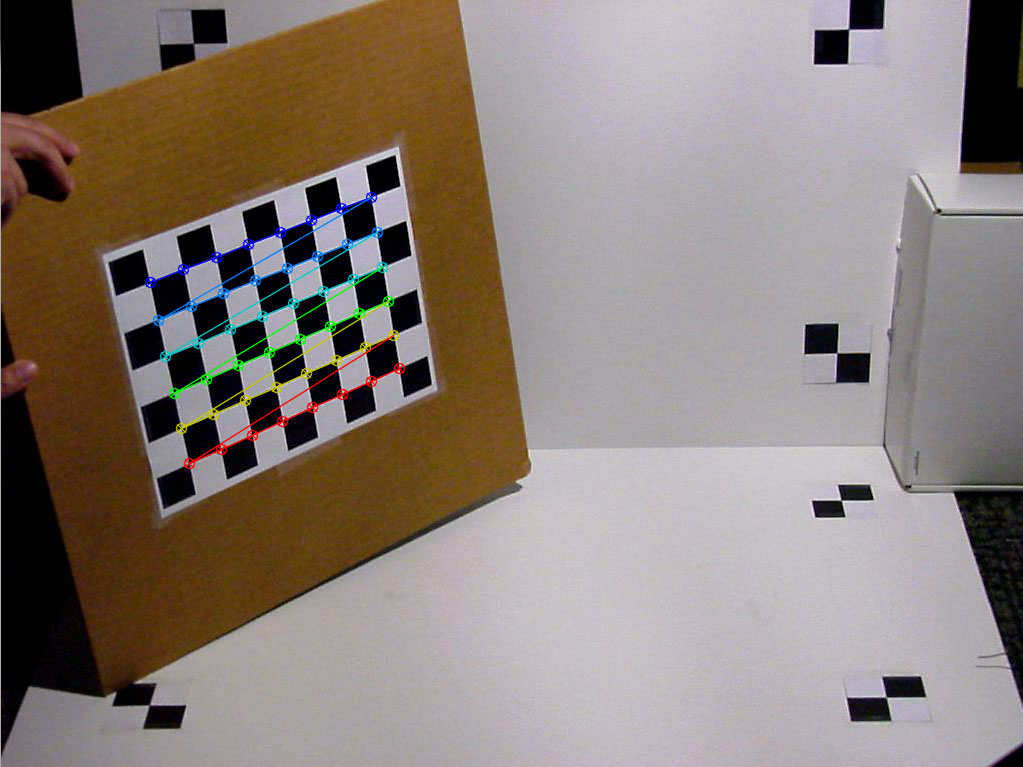
\includegraphics[width=\linewidth]{calib1.jpg}
           
           
    \end{subfigure}
    \begin{subfigure}[b]{0.47\linewidth}
           \centering
            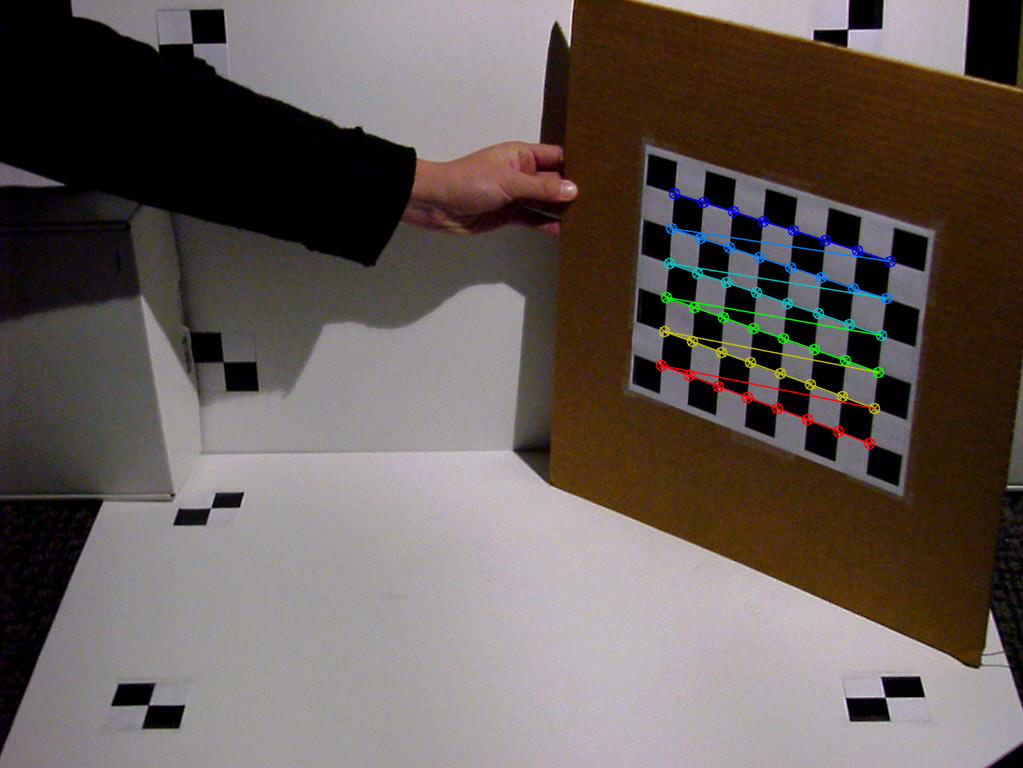
\includegraphics[width=\linewidth]{calib2.jpg}
            
           
    \end{subfigure}
    \caption{Checkerboard images automatically detected.}
 \end{figure}

With the intrinsic parameters the camera ray projecting along each pixel can be computed. To do this, one takes the pixel coordinate, homogenizes it (extending it to a 3D point by having the z value be one), and multiplies this by the inverse of the intrinsic matrix. This resulting point is then multiplied by the camera rotation matrix (taken from the extrinsic parameters), in order to convert the point into world coordinates instead of camera coordinates. Normalizing this point, and using it as the direction from the camera point (also taken from the extrinsic parameters) results in a ray expressed in world coordinates, originating from the camera and being projected out the image plane. 
\begin{figure}[h!]
  \centering
    \begin{subfigure}[b]{0.47\linewidth}
           \centering
            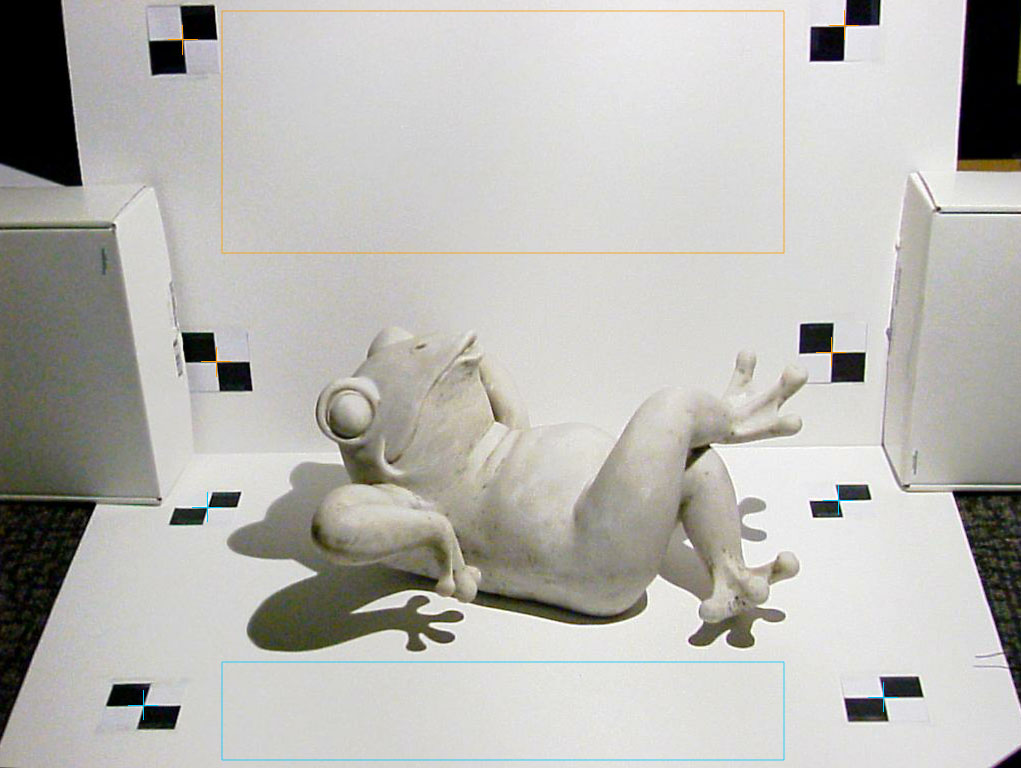
\includegraphics[width=\linewidth]{user_select.jpg}
            
           
    \end{subfigure}
    \caption{User selected pixel to world point correspondences (using measured coordinates of the markers).}\label{userselected}
 \end{figure}

\section{Video Processing}
A first pass of the scanning image sequence is used to generate the min, max, and threshold shadow images. Additionally, a `noise' mask image is created by thresholding to white any pixels whose min value is little different from their max value (effectively, the pixel is in shadow the entire time). This image is used against subsequent frames so no temporal calculations result over these shadowed pixels.
\begin{figure}[h!]
  \centering

    \begin{subfigure}[b]{0.32\linewidth}
           \centering
            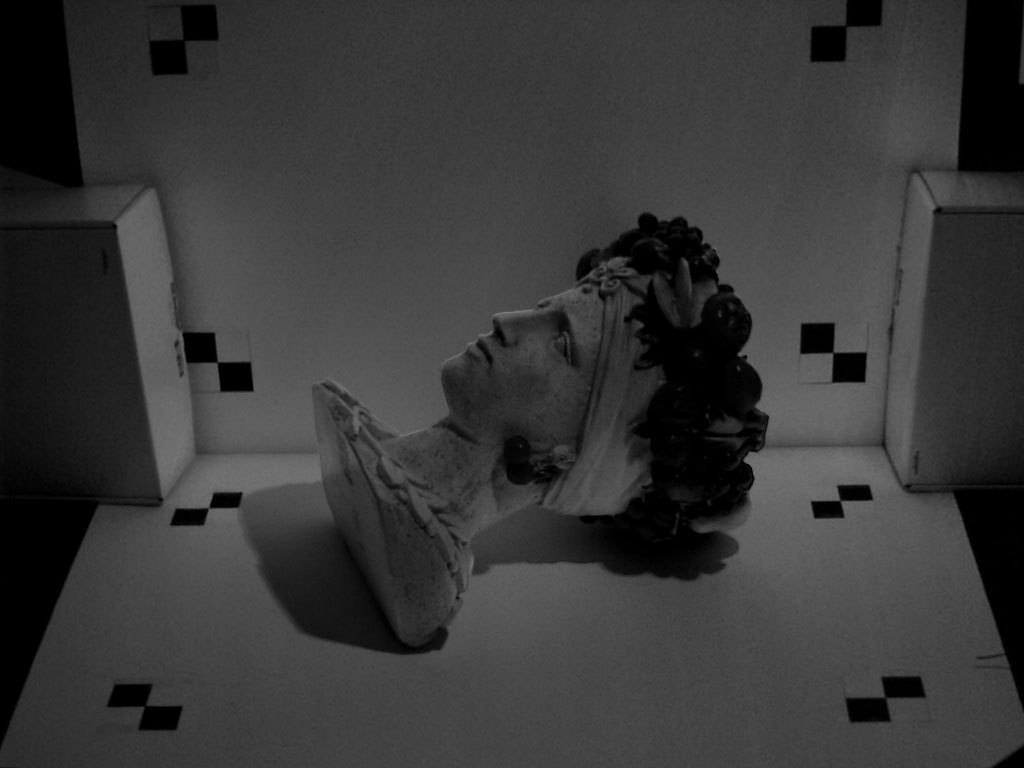
\includegraphics[width=\linewidth]{chiquita/minImg.jpg}           
    \end{subfigure}
    \begin{subfigure}[b]{0.32\linewidth}
           \centering
            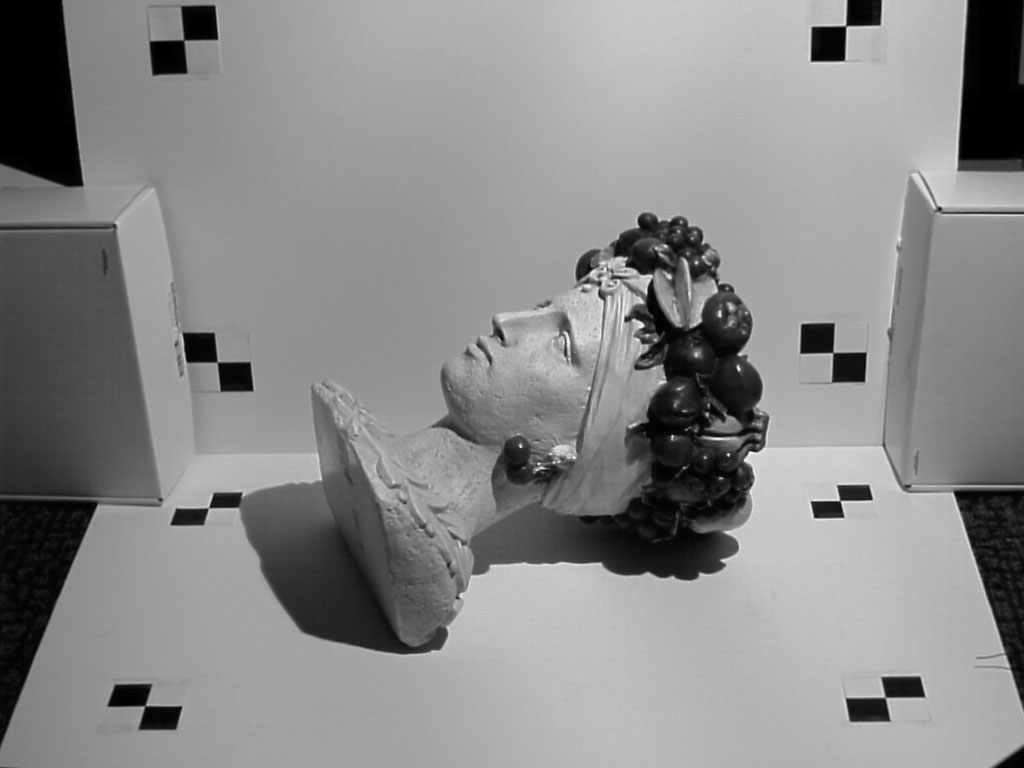
\includegraphics[width=\linewidth]{chiquita/maxImg.jpg}           
    \end{subfigure}
    \begin{subfigure}[b]{0.32\linewidth}
           \centering
            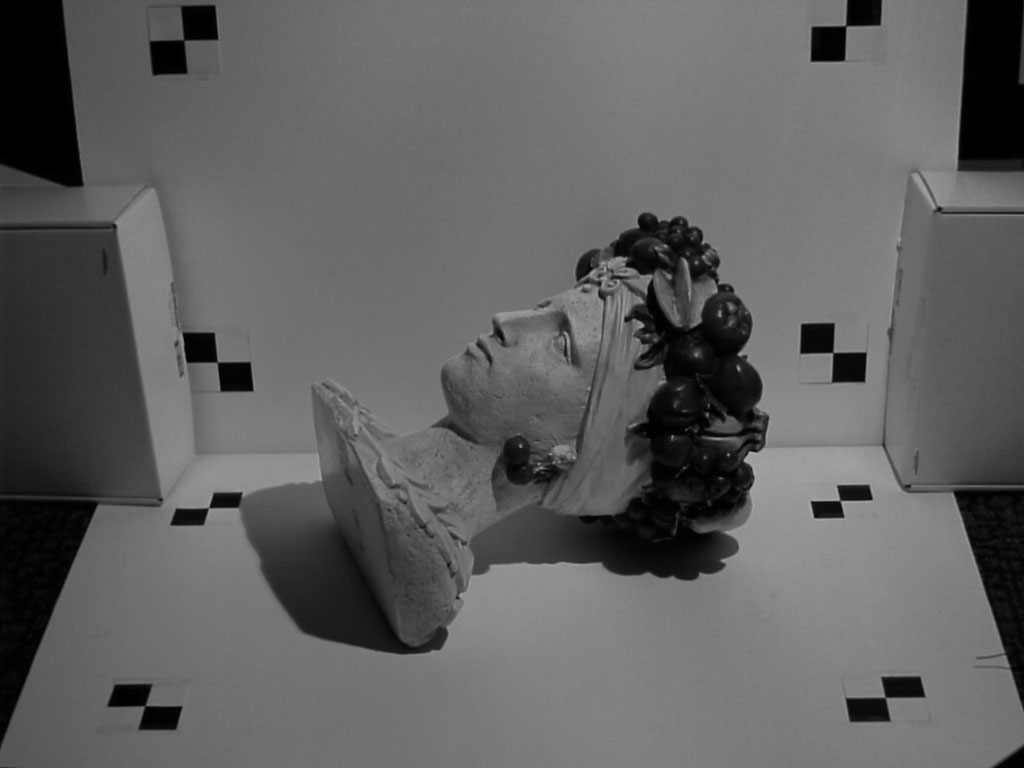
\includegraphics[width=\linewidth]{chiquita/shadowThreshImg.jpg}    
            \end{subfigure}
        \caption{Min, Max , and Average Shadow Threshold images.}\label{}
\end{figure}

\begin{figure}[h!]
  \centering

    \begin{subfigure}[b]{0.32\linewidth}
           \centering
            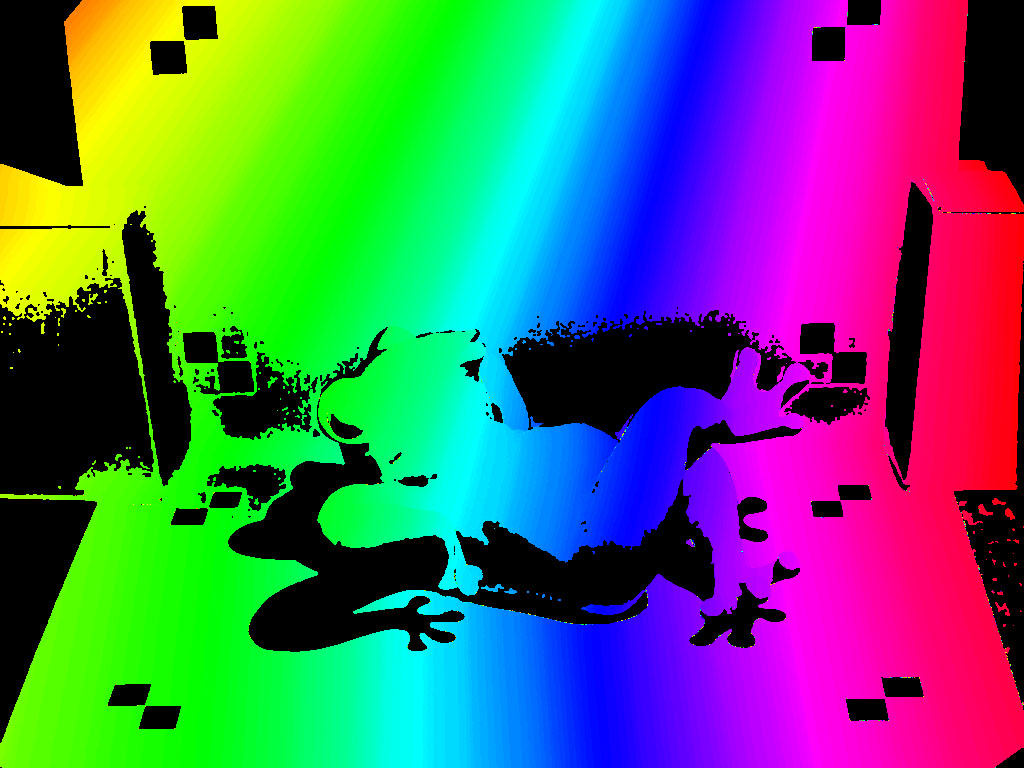
\includegraphics[width=\linewidth]{frog/temporalImg.jpg}
    \end{subfigure}
    \begin{subfigure}[b]{0.32\linewidth}
           \centering
            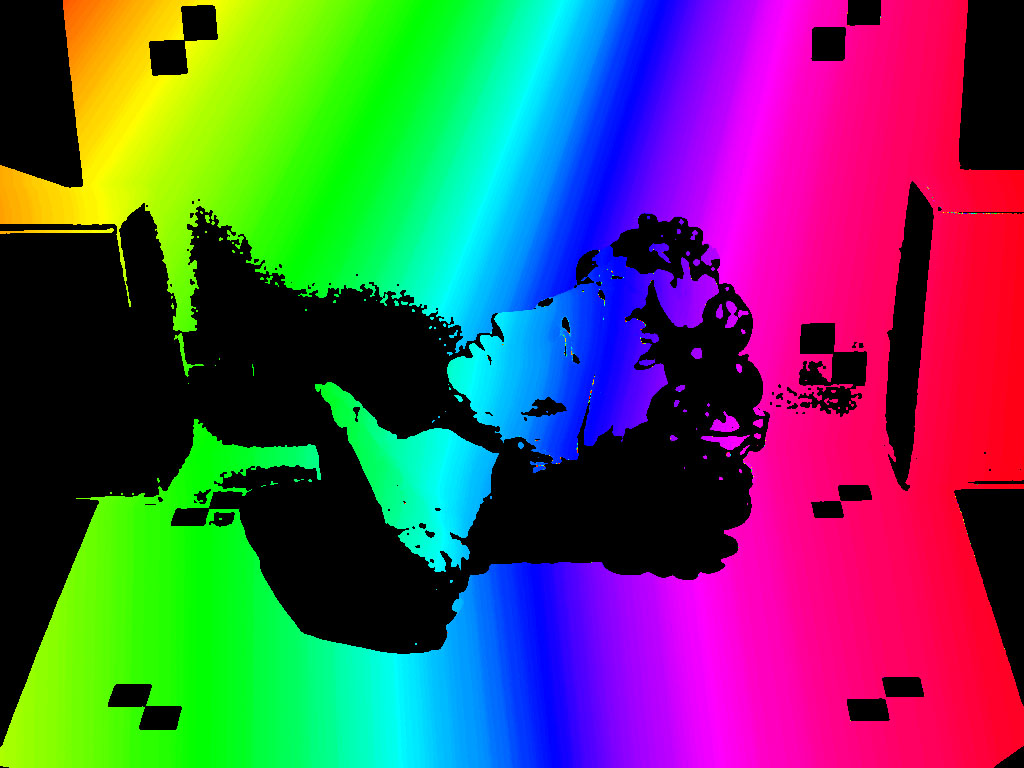
\includegraphics[width=\linewidth]{chiquita/temporalImg.jpg}
    \end{subfigure}
    \begin{subfigure}[b]{0.32\linewidth}
           \centering
            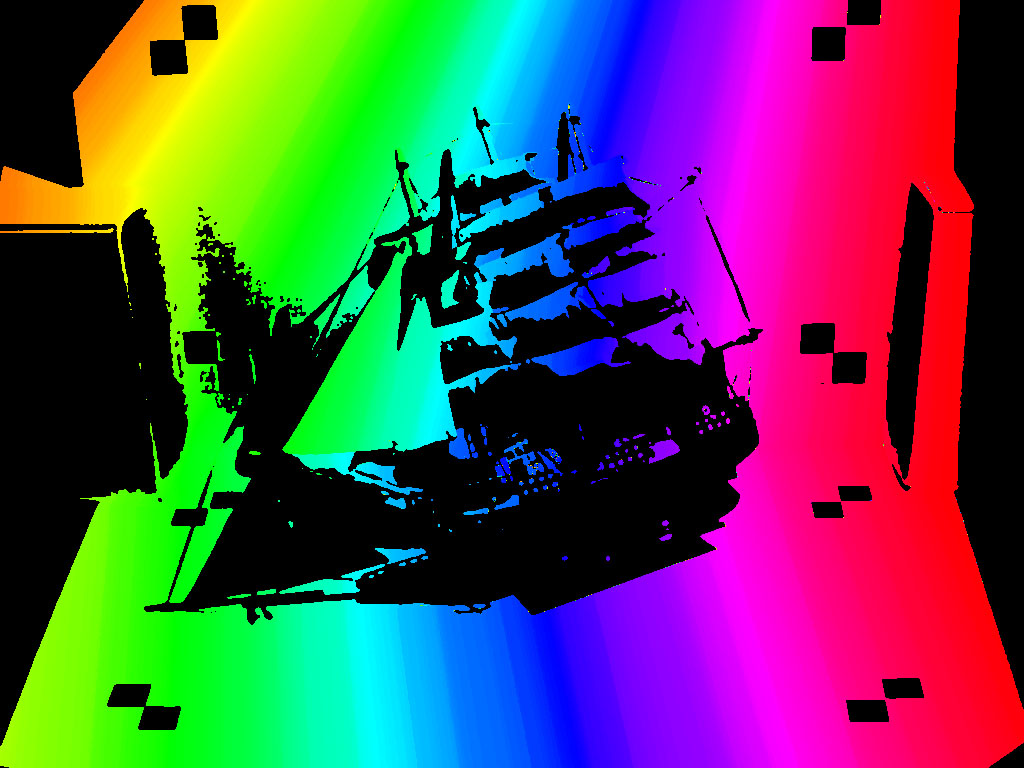
\includegraphics[width=\linewidth]{schooner/temporalImg.jpg}
    \end{subfigure}


        \caption{}\label{}
\end{figure}

\section{Edge Localization}
Using the shadow threshold (and noise mask) images, the zero crossings per frame are computed. The shadow crossings are cropped to user selected boxes (see Figure 3), and the least squares fit 2D shadow crossing line is computed for the vertical and horizontal planes. Projecting these 2D lines mathematically onto the 3D planes results in 2 3D lines (or rays). From the two rays, we can compute the parameterized equation of a plane, the shadow plane. Each plane is stored in a vector indexed by its frame.

Meanwhile, a temporal shadow edge image is generated by mapping the frame index to a color, and setting the pixels currently being shadow-crossed to that color. In this manner, the shadow crossing time (expressed in frames) is stored in each pixel. With the vector of shadow planes indexed by frame number, one can use this information later to retrieve the shadow plane at a specified frame. A function, getPlaneFromFrameIndex(), returns a plane given a frame index. Non-discrete frame values are accepted (say, frame 26.7), and return an interpolated plane.

Blurring and filtering the temporal image resulted in gradient frame values, and reduced some of the noise, but at a loss of resolution of the scan.

\section{Reconstruction and Visualization}
Using the temporal image, the pixel to world ray functionality, and the getPlaneFromFrameIndex() method, we have everything we need to reconstruct the 3D points of the scan. At each pixel in the temporal image, the resulting ray of that pixel is intersected with the resulting plane from the color frame index, creating a 3D point. Rays and planes whose normals are near perpendicular to one another are not intersected, as the tiniest lateral error in their intersection would result in a wildly incorrect point.

Once all 3D points are computed, one can use the tool to view them as a 3D point cloud.
\begin{figure}[h!]
  \centering

    \begin{subfigure}[b]{0.32\linewidth}
           \centering
            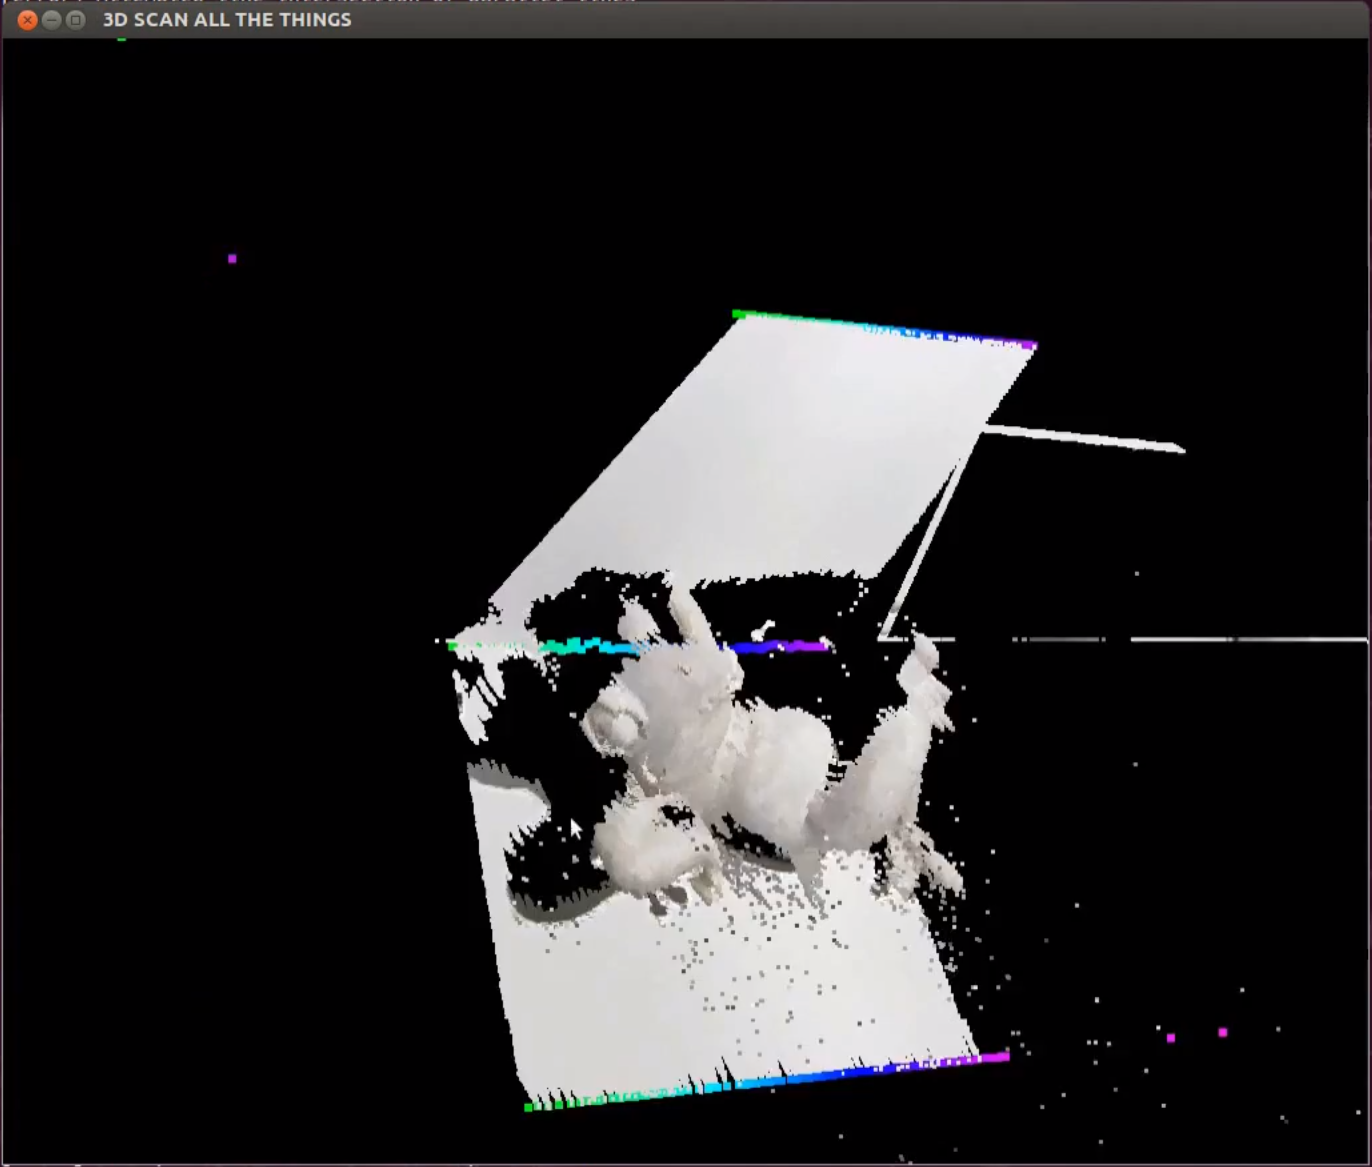
\includegraphics[width=\linewidth]{frog/frog}
            \caption{}
           
    \end{subfigure}
    \begin{subfigure}[b]{0.32\linewidth}
           \centering
            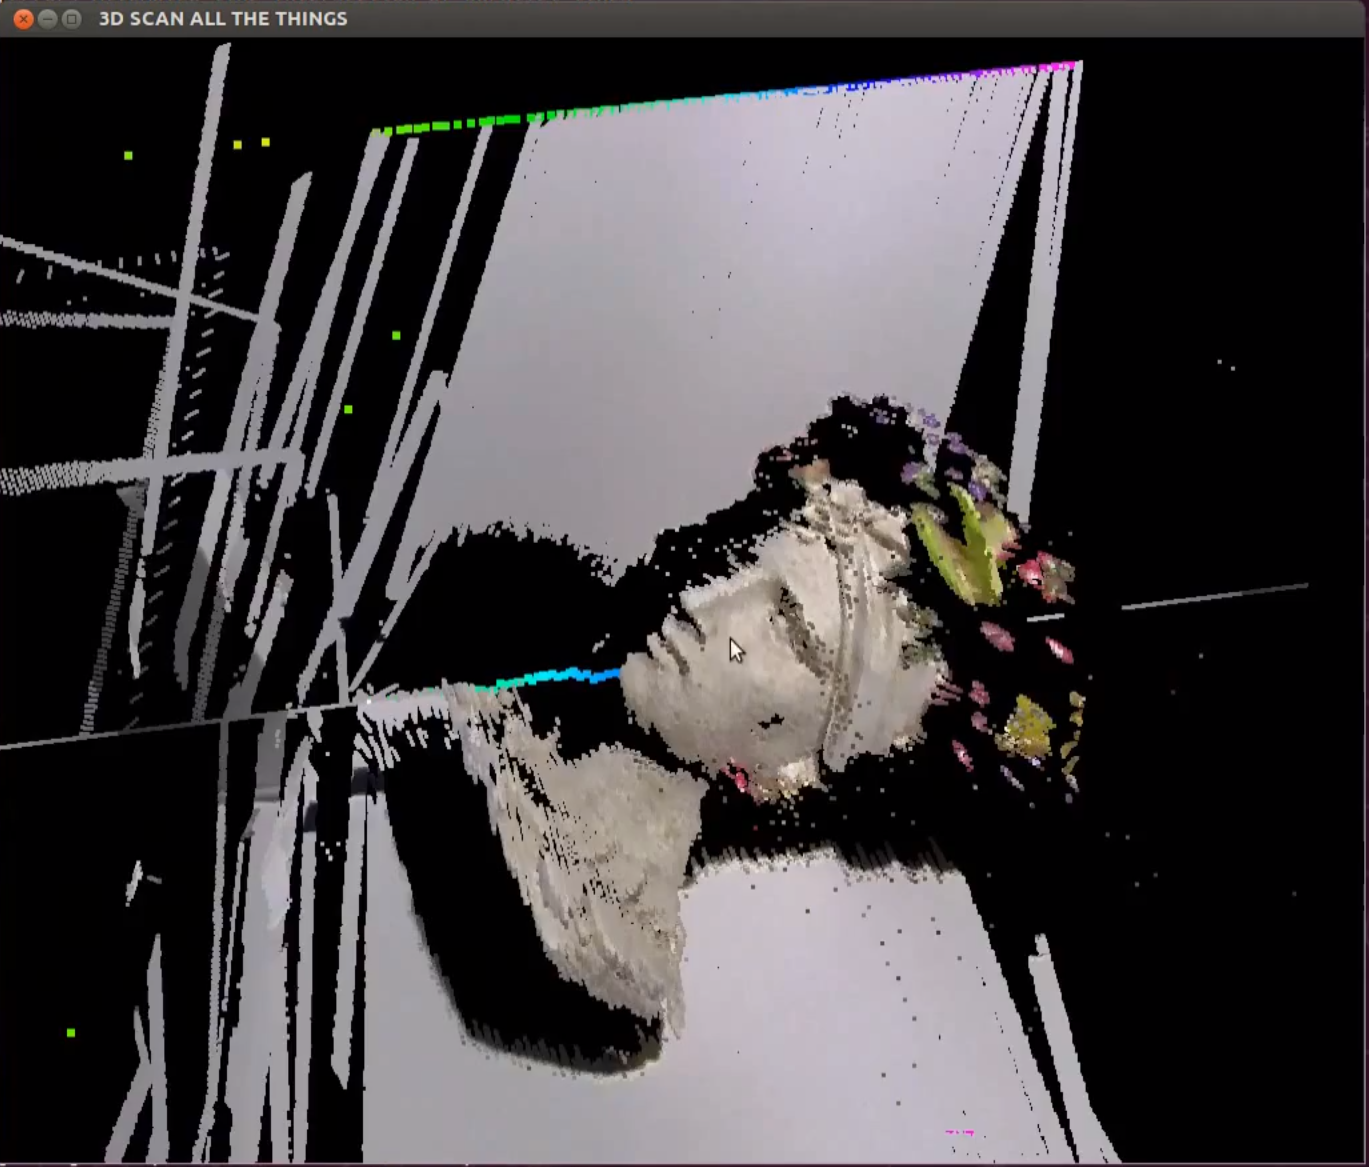
\includegraphics[width=\linewidth]{chiquita/chiquita}
            \caption{}
           
    \end{subfigure}
    \begin{subfigure}[b]{0.32\linewidth}
           \centering
            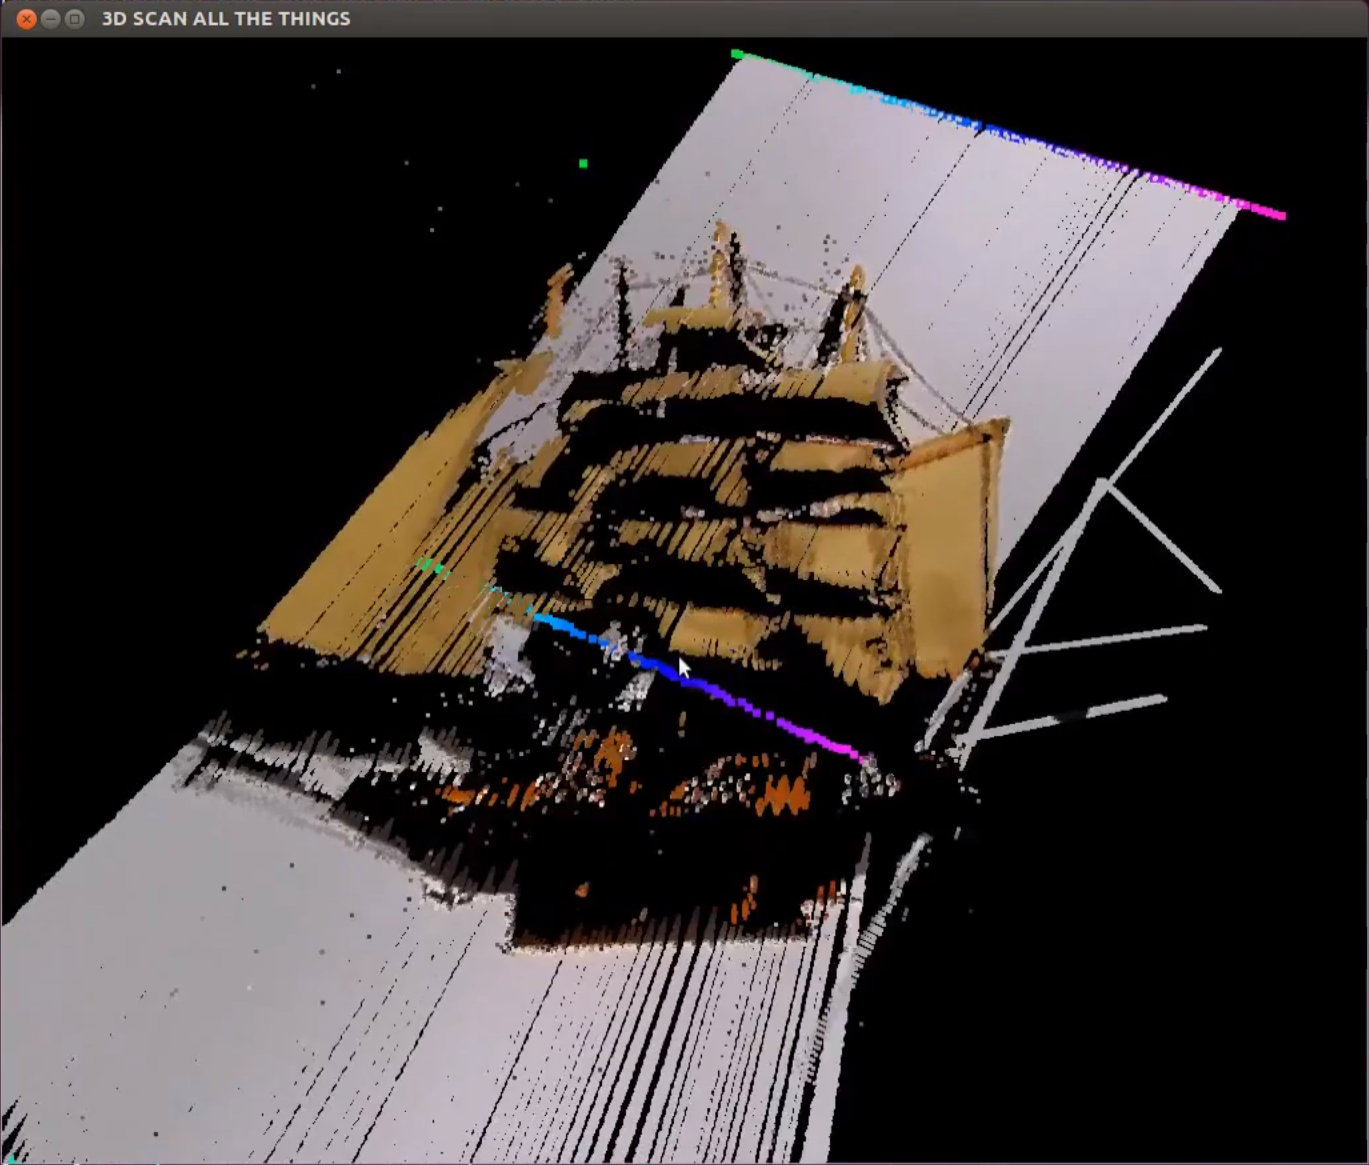
\includegraphics[width=\linewidth]{schooner/schooner}
            \caption{}
           
    \end{subfigure}


        \caption{Scans displayed in the 3D cloud viewer.}\label{}
\end{figure}

Additionally, the 3D points and their colors were outputted as a .ply file format and uploaded to \url{https://sketchfab.com/}. One can view 3 example scanned files at \url{https://sketchfab.com/btparker/recent}.

A video of use cases with the software can be viewed online at \url{http://youtu.be/W98pMUba5Ek}.

One could remove the vertical and horizontal planes from the 3D scan by thresholding the points above a fixed y and z coordinate minimum (as the planes are the xz and xy axis), but I kept them in for framing purposes. However, if consolidating multiple scans they would have to be removed.




%\begin{appendix}
%\section{Supplementary \LaTeX\ Notes}
%
%\end{appendix}

\end{document}





